\documentclass[12pt, oneside]{article} 
\usepackage[a4paper]{geometry}              
\usepackage{graphicx}
\usepackage{amsmath}
\usepackage{amssymb}
\usepackage[table]{xcolor}

%SetFonts
\usepackage[T1]{fontenc}
\usepackage[bitstream-charter]{mathdesign}
%SetFonts

%define example environment 
\newcounter{examplecounter}
\newenvironment{example}%
{%
\small\begin{quote}%
\refstepcounter{examplecounter}%
\textbf{Example \arabic{examplecounter}}%
\quad%
}%
{%\schluss%
\end{quote}%
}

%define remark environment 
\newcounter{remarkcounter}
\newenvironment{remark}%
{%
\small\begin{quote}%
\refstepcounter{remarkcounter}%
\textbf{Remark \arabic{remarkcounter}}%
\quad%
}%
{%\schluss%
\end{quote}%
}

%define remark environment 
\newcounter{questioncounter}
\newenvironment{question}%
{%
\small\begin{quote}%
\refstepcounter{questioncounter}%
\textbf{Question \arabic{questioncounter}}%
\quad%
}%
{%\schluss%
\end{quote}%
}


%define important environment
\newenvironment{important}{\begin{quote}%
\textbf{Important:}%
\quad
}{%
\end{quote}%
}

\newcommand{\qed}{\nobreak \ifvmode \relax \else
      \ifdim\lastskip<1.5em \hskip-\lastskip
      \hskip1.5em plus0em minus0.5em \fi \nobreak
      \vrule height0.5em width0.5em depth0.25em\fi}

\newtheorem{theorem}{Theorem}[section]
\newtheorem{lemma}[theorem]{Lemma}
\newtheorem{proposition}[theorem]{Proposition}
\newtheorem{definition}{Definition}
\newenvironment{proof}[1][Proof]{\begin{trivlist}
\item[\hskip \labelsep {\bfseries #1}]}{\end{trivlist}}

\newcommand{\R}{\mathbb{R}}
\newcommand{\E}{\mathbb{E}}
\newcommand{\fol}{\mathcal{F}}
\newcommand{\one}{\mathbb{1}}
\newcommand{\hest}{\textsc{Hesten}}
\newcommand{\texp}{T_{\rm exp}}

\usepackage{lettrine}

\begin{document}
\noindent{\Huge \textbf\textsf{{Completing the correlation matrix in a hybrid model.}}}

\noindent \textit{by Horst K�hler, Thomas Streuer, Olaf Dreyer}

\vspace{.5cm}

\section{Introduction}

\section{The cross currency model}
To make the issues more concrete we introduce the basic cross currency model as an example. This model consists of two interest rate models and a model for the exchange rate. We will denote the base currency by $E$ and assume that we model a rate $x_E$ together with a volatility $\nu_E$. The details of the model are not important since we are only concerned about the correlation of the stochastic processes. An example of such a model would be a Heath-Jarrow€-Morton model with a stochastic volatility. The model for the foreign currency $A$ will also consist of a model for the rate $x_A$ and the volatility $\nu_A$. The remaining model will be for the exchange rate 
\begin{equation}
	X_E^A,
\end{equation}
where the lower index $E$ denotes the currency we are converting into and the upper index is the currency we are converting from. If $m_A$ is an amount in currency $A$ then
\begin{equation}
	X_E^A m_A
\end{equation}
is the corresponding amount in the currency $E$. We also assume that we are modeling the volatility $\nu_{EA}$ of the exchange rate. An example of such a model would be a Heston model \cite{heston}. Altogether we thus have these six stochastic variables:
\begin{equation}
	x_E, \nu_E, x_A, \nu_A, X_E^A, \nu_{EA}
\end{equation}
Let us denote this set of variables by $I$. For two elements $a,b\in I$ let 
\begin{equation}
	(a,b) = \langle W_a, W_b\rangle
\end{equation}
be the correlation coefficient\footnote{We introduce this non-standard notation here to improve the readability in later chapters.} for the stochastic processes of $a$ and $b$. For all $a,b\in I$ we have
\begin{align}
	(a,b) & = (b,a) \\
	(a,a) & = 1\\
	\vert(a,b)\vert & \le 1
\end{align}
In principle one could imagine that all entries of $W$ are determined in one calibration using an assortment of financial products. This is usually not what one does though because the number of parameters is too large and hence the calibration is too unstable but also because one will have already performed calibrations for the interest models themselves and thus
\begin{equation}
	(x_E, \nu_E)\text{\ and\ }(x_A, \nu_A)
\end{equation}
are already known. In addition to these two, one might decide to calibrate the coefficients
\begin{equation}
	(x_E, X_E^A),(x_E, x_A), (x_A, X_E^A)\text{, and\ } (X_E^A, \nu_{EA}).
\end{equation}
The question that arises is then how to determine the remaining coefficients (see figure \ref{fig.xccymodel} of the correlation matrix.

\begin{figure}[hbt]
  \begin{center}
  	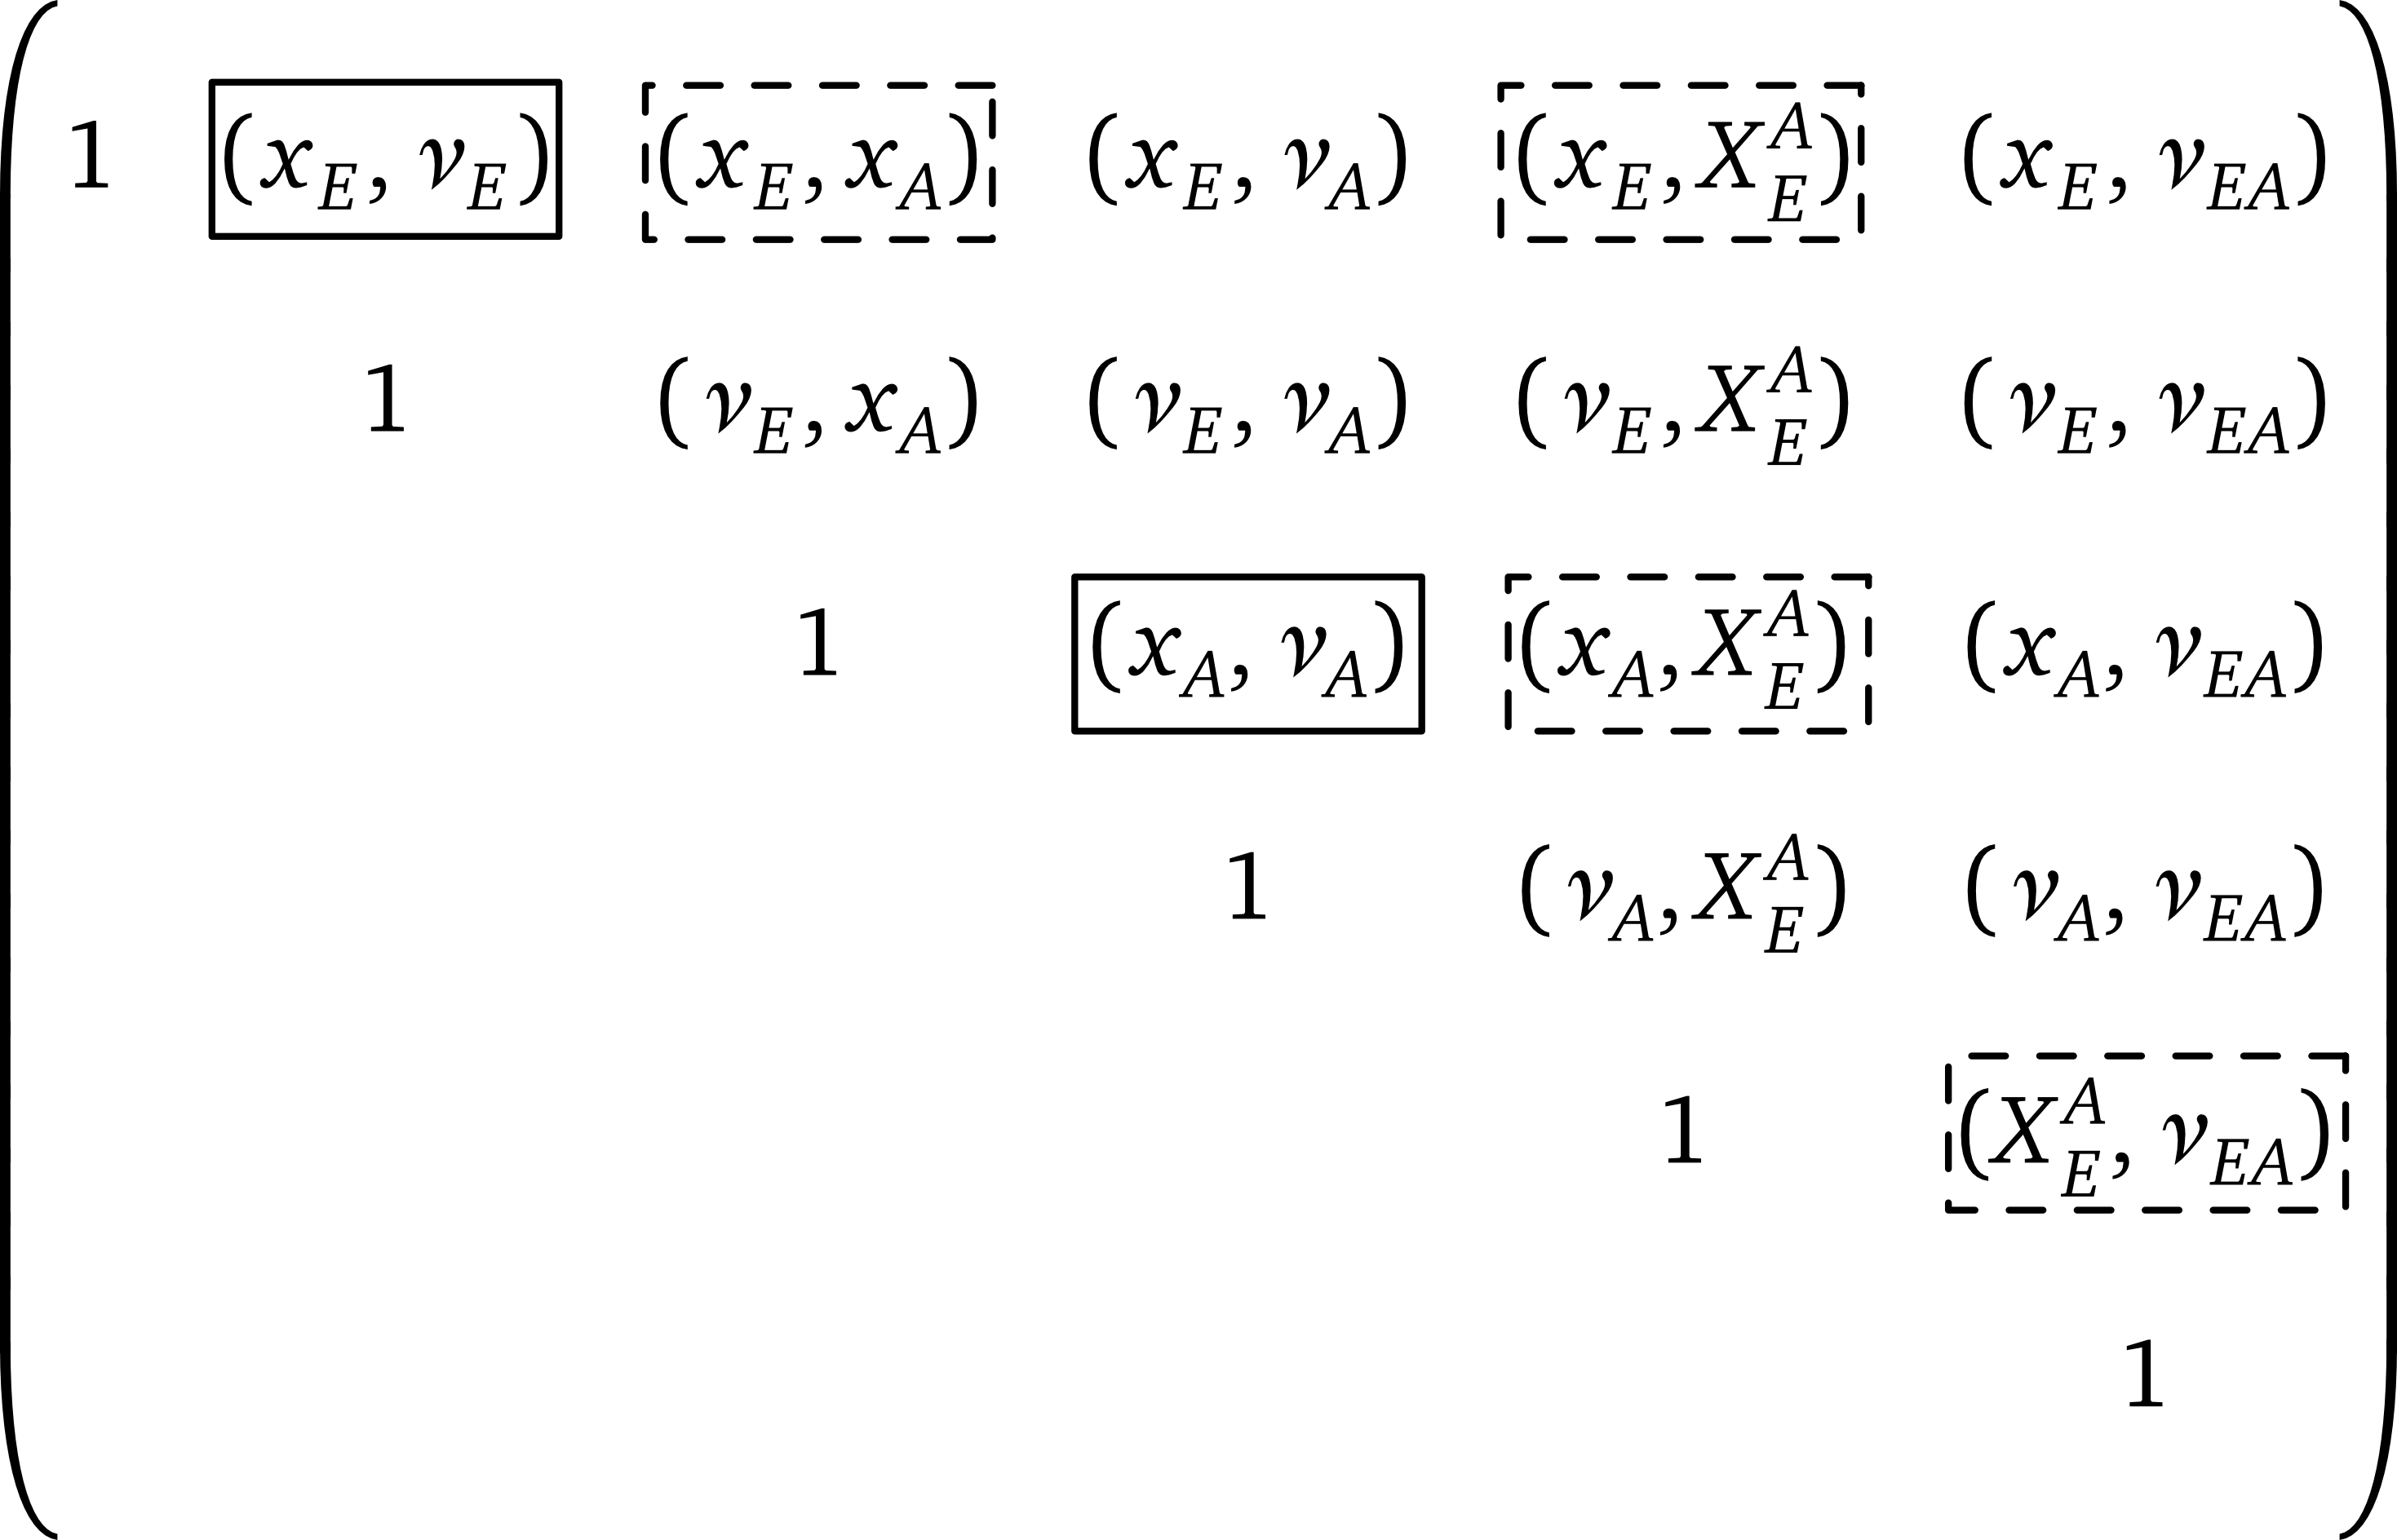
\includegraphics[width=10cm]{img/xccymodel.png}
  \end{center}
  \caption{The correlation matrix for the cross currency model. The coefficients $(x_E, \nu_E)$ and $(x_A, \nu_A)$ (the boxes with the solid lines) will be determined in two separate interest rate calibrations. The coefficients $(x_E, X_E^A)$, $(x_E, x_A)$, $(x_A, X_E^A)$, and $(X_E^A, \nu_{EA})$ (the boxes with the dashed lines) will be determined in the cross currency calibration. The question then arises what to do witht he remaining coefficients?}\label{fig.xccymodel}
\end{figure}

\section{Independence, maximal determinant, and entropy}
Before we answer the question of the last section in full generality we look at a simpler case. 


\section{The completion procedure}

\section{The general hybrid model}

\begin{thebibliography}{MM}
	\bibitem{heston} Steven L. Heston, A Closed-Form Solution for Options with Stochastic Volatility with Applications to Bond and Currency Options, The Review of Financial Studies, \textbf{6}(2), April 1993, 327--343.
\end{thebibliography}


\end{document}